\subsection{Vulnerabilità}

\begin{frame}
    Le vulnerabilità trovate negli anni nel critto-sistema sono le seguenti.

    Alcune di queste sono di facile soluzione perché riguardano il lato hardware del lettore,
    per cui, a fronte di un costo maggiore, è possibile migliorarne le capacità.
\end{frame}

\begin{frame}
    \frametitle{Vulnerabilità}
    \scriptsize
    \begin{enumerate}
        \item <1-> Utilizzo di chiavi a 48 bit: Possibili attacchi BruteForce \cite{courtois2008algebraic}\label{enum:keylength}
        \item <2-> RNG del tag non è crittograficamente sicuro. Infatti è un LFSR (a 16 bit)~\cite{garcia2008dismantling} con condizione iniziale costante.\label{enum:rng-16-bit}
        \begin{enumerate} \scriptsize
            \item <3-> Consegue che lo stato è prevedibile e dipende dal tempo trascorso dal power-on~\cite{garcia2008dismantling}\cite{courtois2008algebraic}\label{enum:rng-constant-seed}
            \item <4-> Inoltre i numeri casuali sono generati a partire da 16 bit del registro 
            \item <5-> In particolare i numeri sono generati ad ogni ciclo di clock del tag, quindi la precisione dell' attaccante deve limitarsi a quanti di 10 microsecondi (106kHz) e la sequenza di numeri si ripete ogni 65535 iterazioni (0.6s)
        \end{enumerate}
        \item <6-> L'RNG dei lettori viene aggiornato solamente ad ogni nuova autenticazione~\cite{garcia2008dismantling}\label{enum:rng-reader-update}
        \item <7-> La funzione di filtraggio del LFSR usa 20bit del registro e sono solo bit in posizione dispari
        \item <8-> LFSR State Recovery
        \item <9-> LFSR Rollback
        \item <10-> I bit di parità sono computati sul plaintext e poi inviati non cifrati
    \end{enumerate}
\end{frame}
\note{
    \ref{enum:keylength} L'unica protezione contro attacchi bruteforce sta nel tempo di transazione di alcuni millisecondi ma non c'è nessuna protezione da attacchi su ciphertext.

    \ref{enum:rng-16-bit} Dalla analisi dei pacchetti è stato possibile notare che lo stato del RNG è di soli 16 bit. 
    Questo comporta l'esistenza di soli 65536 possibili nonce e che la seconda parte di $n_t$ sia funzione della prima. In particolare è stato possibile identificare che un nonce è valido se e solo se è rispettato \[n_k \oplus n_k+2 \oplus n_k+3 \oplus n_k+5 \oplus n_k+16 = 0\]

    \ref{enum:rng-16-bit}.\ref{enum:rng-constant-seed} Tramite tentativi e analisi dei dati trasmessi è stato possibile rilevare che il valore del nonce $n_t$ dipende solamente dal tempo di accensione del tag.
    Questo permette di evincere che il generatore di numeri casuali ha un seed iniziale codificato nell'hardware.

    \ref{enum:rng-reader-update} Questo implica che possono esistere numerosi lettori vulnerabili ad attacchi sul parametro $n_r$, infatti è possibile notare che la sequenza dei nonce $n_r$ a partire dall'avvio del lettore non varia.
}

\begin{frame}
    \frametitle{Funzione di filtraggio dipendente da bit in posizione dispari}
    La funzione di filtraggio è stata identificata ed è stato notato come solo i bit in posizione dispari siano input ad essa. \pause

    I bit dispari dello stato sono responsabili della codifica dei bit dispari del messaggio\pause
    
    I bit pari dello stato sono responsabili della codifica dei bit pari del messaggio
\end{frame}
\note{
    È così possibile ricostruire lo stato a partire da un keystream dividendo l'identificazione in due processi paralleli, uno che permetterà di trovare i bit pari e uno i bit dispari.

    Per precisione, siano $b_0, b_1, b_2 ... b_{n-1}$ i bit del keystream (per un numero pari di bit, dato che i messaggi hanno sempre lunghezza pari).
    Bisogna trovare la sequenza $\bar{r} = r_0, r_1, r_2 ... r_{46+n}$ tale per cui valga la relazione 
    \begin{multline*}
        r_k \oplus r_k+5 \oplus r_k+9 \oplus r_k+10 \oplus r_k+12 \oplus r_k+14 \oplus r_k+15 \oplus r_k+17 \\
\oplus r_k+19 \oplus r_k+24 \oplus r_k+25 \oplus r_k+27 \oplus r_k+29 \oplus r_k+35 \oplus r_k+39 \oplus r_k+41 \\
\oplus r_k+42 \oplus r_k+43 \oplus r_k+48 = 0\\ \forall k \in \{0, . . . , n - 2\}
    \end{multline*}
    e tale che \[f(r_k . . . r_k+47 ) = b_k, \forall k \in \{0, . . . , n - 1\}. \]

    In questo modo tutte le sotto sequenze di $\bar{r}$ di lunghezza 48 saranno stati in successione del LFSR
}

\begin{frame}
    \frametitle{Bit di parità}
    \label{sec:parity-enc}
    Ulteriore vulnerabilità dell'implementazione è il fatto che il livello di trasmissione fisica richiede 
    un invio di un bit di parità ogni 8 bit di dato

    IL BIT DI PARITÀ È QUINDI INVIATO CIFRATO \textbf{CONDIVIDENDO IL BIT DEL KEYSTREAM} MA VIENE \textbf{CALCOLATO SUL PLAINTEXT}\cite{Courtois2009TheDS}

    \begin{figure}
        \centering
        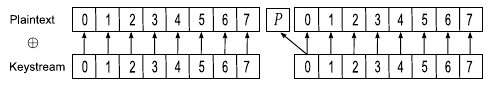
\includegraphics[width=0.8\textwidth]{keystream-parity.png}
        \caption{Assegnazione dei bit di cifratura tra dati e bit di parità}
        \label{fig:keystream-parity}
    \end{figure}
\end{frame}
\note{
    Questo permette di avere informazioni sul keystream (almeno su un bit ogni 8) ed è una proprietà utilizzabile per ridurre lo spazio di ricerca negli attacchi Nested authentication (vedi slide~\ref{sec:nested-auth})
}

\begin{frame}
    \frametitle{Errori di trasmissione}
    \label{sec:parity-bit-vuln}
    Secondo il protocollo ISO14443a ogni 8 bit di dati deve essere inviato un bit di parità.\pause

    Il tag riceve una sequenza di dati con bit di parità invalidi $\implies$ Nessuna risposta da parte del tag\pause

    Il tag riceve una sequenza con bit di parità corretti ma la verifica della risposta alla challenge non ha successo $\implies$ NACK\pause

    {\large IL NACK È CIFRATO MA È UN TESTO CONOSCIUTO}
\end{frame}
\note{
    Questo permette, dopo aver collezionato un buon quantitativo di NACK, di attaccare il cifrario tramite inversione della funzione di filtraggio e il successivo rollback.
}